%\chapter{Desenvolvimento}
\label{desenvolvimento}
\section{Remoção na SBB Sequencial}
    Iniciando o desenvolvimento da prática, as arvores foram criadas na IDE assim como os vetores de tamanhos diversos para armazenar os valores que serão inseridos na arvore. Porém, o Java não permite a criação de vetores em 10\textsuperscript{9} elementos, então todas as arvores criadas, foram geradas até 10\textsuperscript{7} elementos. A partir disso, foram utilizados métodos de inserção de dados da Pratica 3, desenvolvida anterior a esta, já que este trabalho trata-se de uma continuação direta com estudos sobre remoção.
    
    Aos dados selecionados para a remoção foram gerados utilizando a biblioteca interna do Java "Random", que permitiu gerar valores aleatórios entre 0 e n (n = quantidade de elementos), aumentando a taxa de sucesso para gerar valores validos para a remoção.
    Os dados apresentados a seguir inicialmente trazem os resultados do tempo de execução da da remoção de 5\% de elementos aleatórios de arvores de diferentes tamanhos que receberam seus valores de forma ordenada:
    
    \begin{center}
        \begin{tabular}{| l | r |}
            \hline
            Quantidade de elementos & Tempo em Nanossegundos\\
            \hline
            10\textsuperscript{3} & 820800\\
            10\textsuperscript{5} & 2165600\\
            10\textsuperscript{7} & 119273300\\
            \hline
        \end{tabular}
    \end{center}

        \begin{center}
            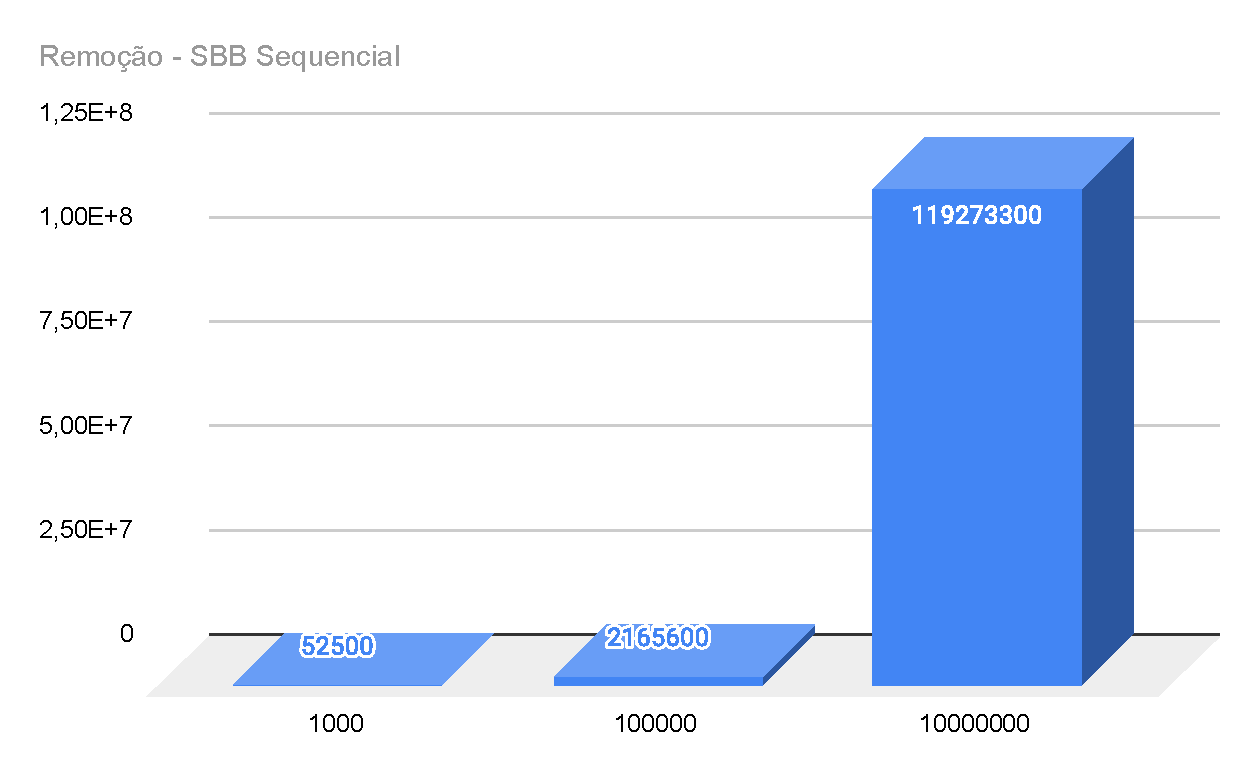
\includegraphics[scale=0.8]{Trabalho AED/fig/chart.pdf}
            \label{fig:Grafico 1}
        \end{center}

\section{Remoção na SBB Randômica}

Para a remoção de elementos aleatórios desta arvore foi gerado um vetor com valores aleatórios utilizando um gerador congruencial pseudo aleatório com os seguintes parâmetros:
        \begin{center}
        Semente = 0;
       
        Modulo = 1073741824;
       
        Multiplicador = 843314861;
       
        Incremento = 453816693;
        \end{center}

Estes parâmetros também foram utilizados na inserção, então é certo que os mesmos estarão na arvore, mas não foram removidos na mesma ordem que foram inseridos, e sim de forma aleatória também.

Logo os dados apresentados a seguir trazem os resultados do tempo de execução da da remoção de 5\% de elementos aleatórios de arvores de diferentes tamanhos que receberam seus valores de forma aleatória:

\begin{center}
        \begin{tabular}{| l | r |}
            \hline
            Quantidade de elementos & Tempo em Nanossegundos\\
            \hline
            10\textsuperscript{3} & 208600\\
            10\textsuperscript{5} & 3452300\\
            10\textsuperscript{7} & 822413400\\
            \hline
        \end{tabular}
    \end{center}
    
    \begin{center}
            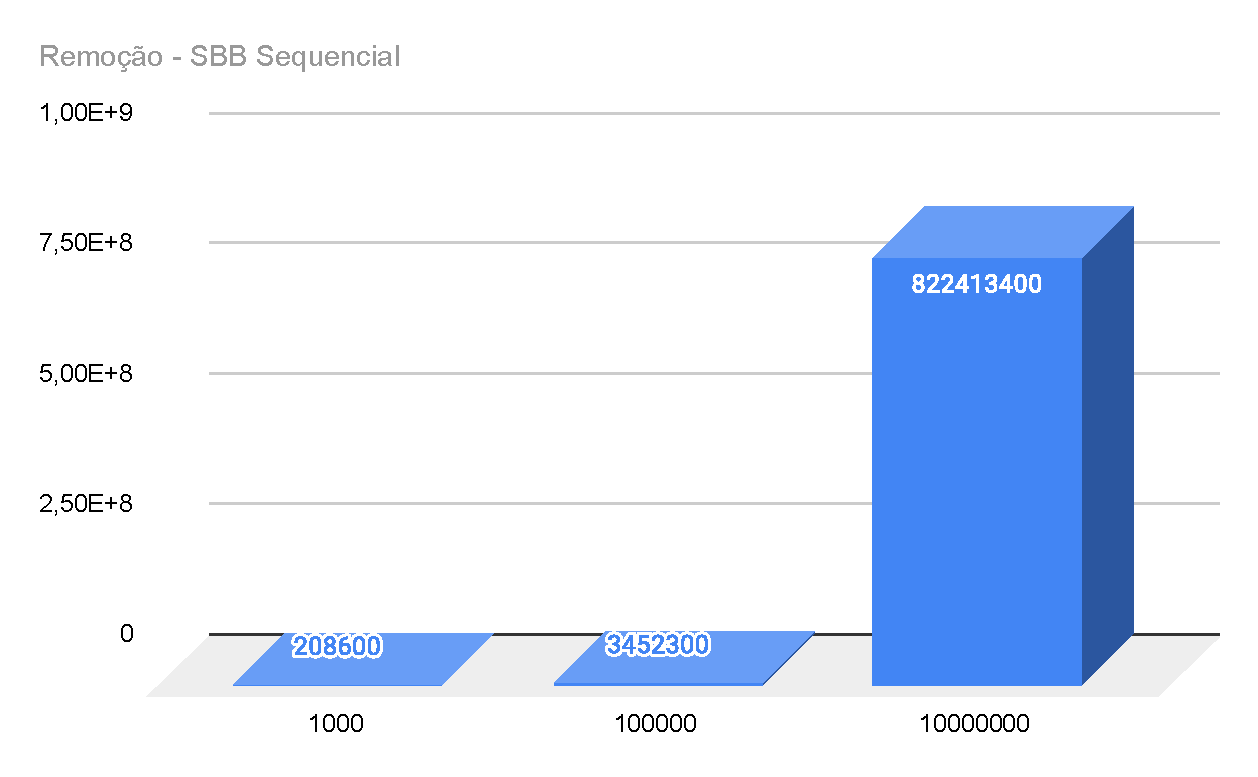
\includegraphics[scale=0.8]{Trabalho AED/fig/chart (1).pdf}
            \label{fig:Grafico 2}
    \end{center}
    
\section{Remoção na SBB Balanceada}
Para a remoção de elementos de dentro da arvore balanceada a logica utilizada segue a mesma da arvore sequencial, já que os valores inseridos na mesma estão entre 0 e n (n = quantidade de elementos), porem foram inseridos em uma condição especial que força a arvore a ser formada de já balanceada, como foi visto na atividade pratica 3.

Logo os dados apresentados a seguir trazem os resultados do tempo de execução da remoção de 5\% de elementos aleatórios de SBBs de diferentes tamanhos:

    \begin{center}
        \begin{tabular}{| l | r |}
            \hline
            Quantidade de elementos & Tempo em Nanossegundos\\
            \hline
            10\textsuperscript{3} & 11700\\
            10\textsuperscript{5} & 769600\\
            10\textsuperscript{7} & 149937300\\
            \hline
        \end{tabular}
    \end{center}
    
    \begin{center}
            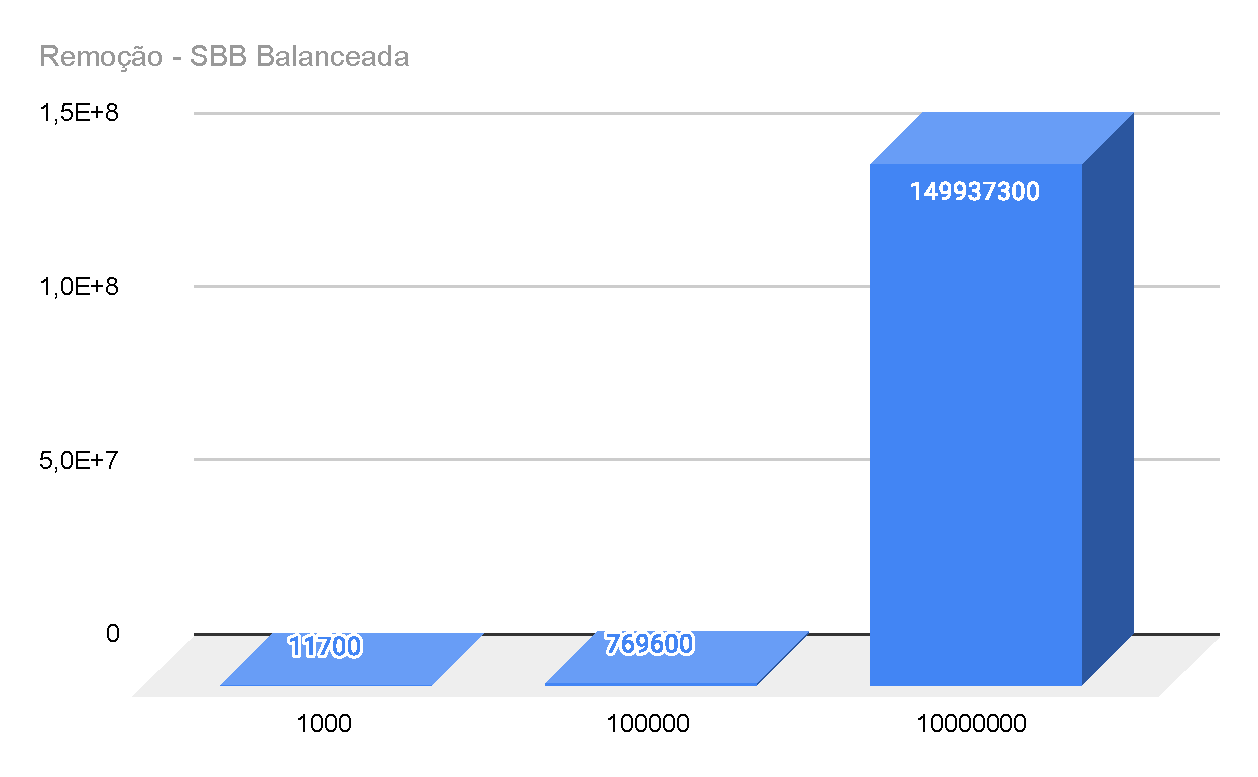
\includegraphics[scale=0.8]{Trabalho AED/fig/chart (2).pdf}
            \label{fig:Grafico 3}
    \end{center}
    
\section{Busca de elementos na TRIE}
Para a execução dos testes neste modelo de estrutura de dados foi utilizada uma implementação\cite{Samuellucas97} que recebe palavras no formato de String e as compara de acordo com seu tamanho e prioridade em ordem alfabética e facilitar a implementação de grandes quantidades de palavras foi implementado um gerador de Strings aleatórias, que utiliza de um vetor com todas as lestras do alfabeto que este método seleciona posições aleatórias do vetor e gera uma String com as letras destas posições\cite{gerarString}.

Logo os dados apresentados a seguir trazem os resultados do tempo de execução da
busca de 1\% de elementos aleatórios de TRIEs de diferentes tamanhos:

\begin{center}
        \begin{tabular}{| l | r | r | r | }
            \hline
            Quantidade de elementos & Elementos Buscados & Media de Tempo & Desvio Padrão\\
            \hline
            10\textsuperscript{3} & 100 & 1230 & 6845,509\\
            10\textsuperscript{5} & 1000 & 471,5 & 9743,600\\
            10\textsuperscript{7} & 100000 & 353,57 & 132471,980\\
            \hline
        \end{tabular}
    \end{center}

\begin{center}
            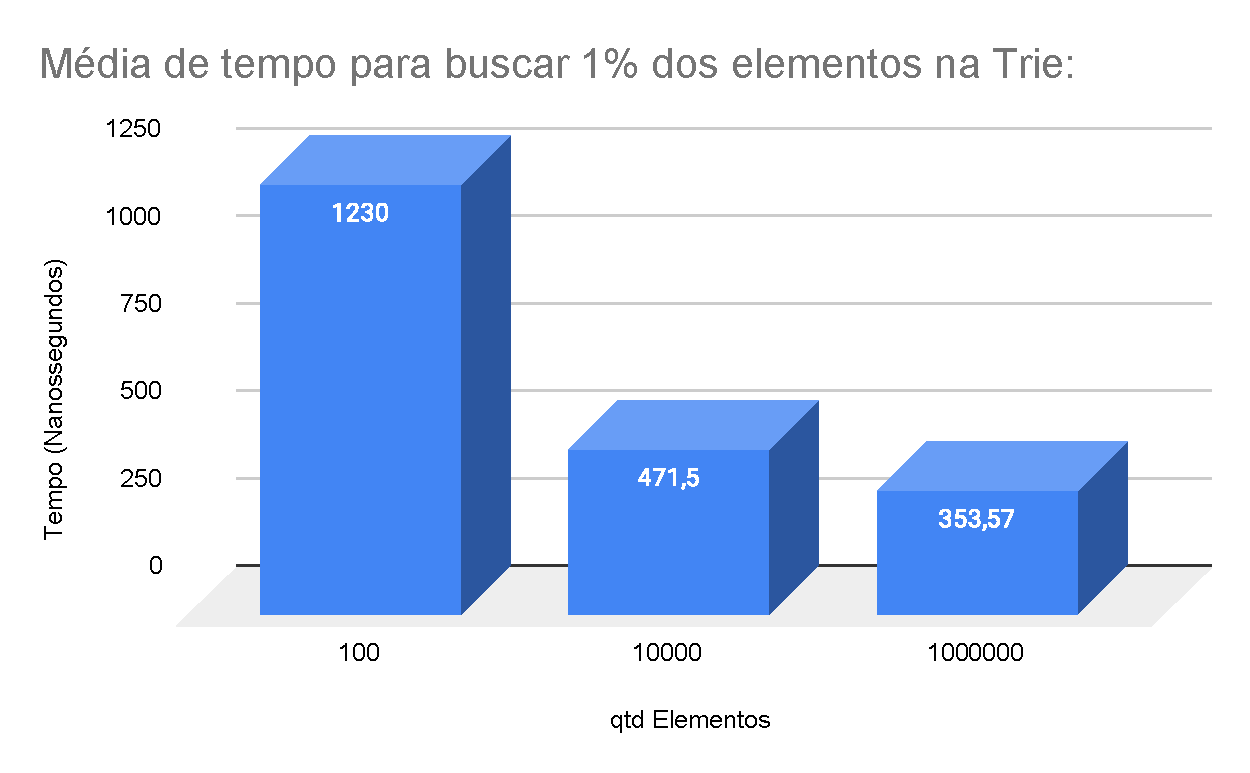
\includegraphics[scale=0.7]{Trabalho AED/fig/MediaTrie.pdf}
            \label{fig:Media de tempo Trie}
    \end{center}
    
\begin{center}
            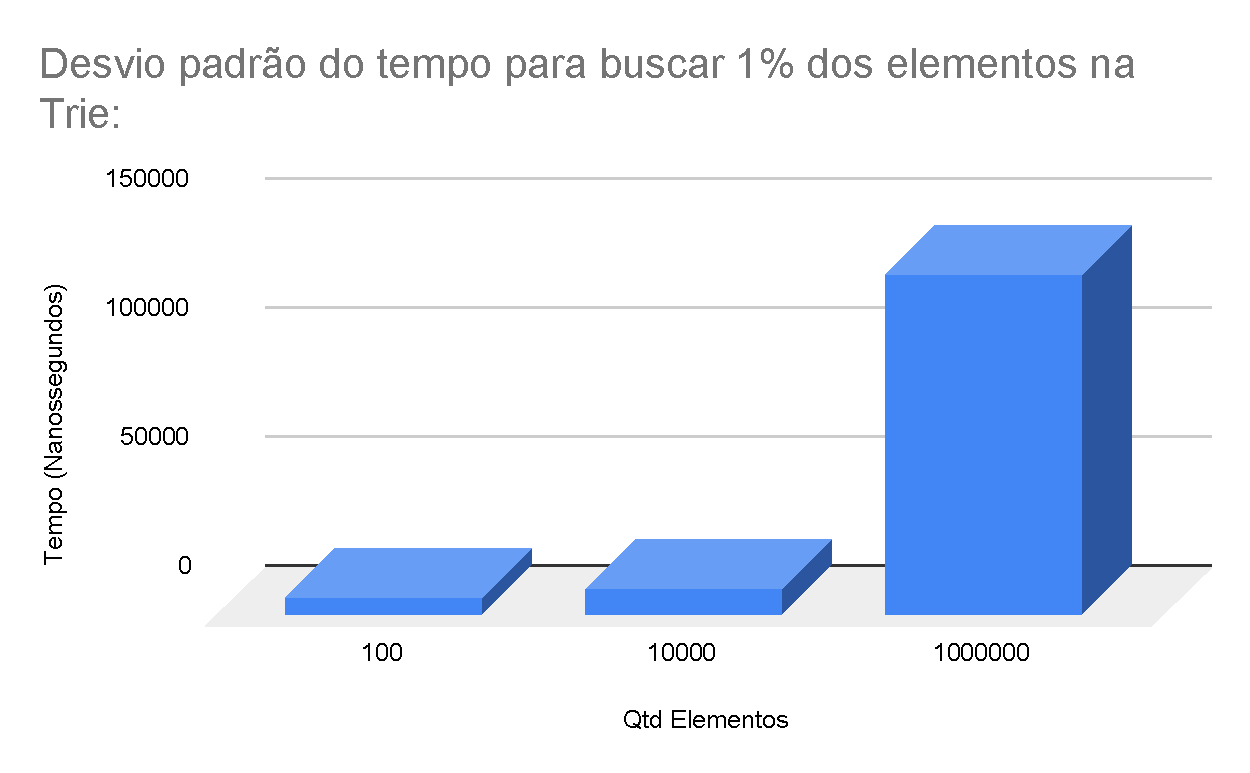
\includegraphics[scale=0.7]{Trabalho AED/fig/DesvioTrie.pdf}
            \label{fig:Media de tempo Trie}
    \end{center}

\section{busca de elementos na PATRICIA}

Para execução dos testes neste modelo de dados foi utilizado uma implementação que recebe inteiros no no formato de Interger e os compara byte a byte\cite{nivioziviani}.

Logo os dados apresentados a seguir trazem os resultados do tempo de execução da
busca de 1\% de elementos aleatórios de Patricia de diferentes tamanhos:

\begin{center}
        \begin{tabular}{| l | r | r | r | }
            \hline
            Quantidade de elementos & Elementos Buscados & Media de Tempo & Desvio Padrão\\
            \hline
            10\textsuperscript{3} & 100 & 980,0 & 2572,158626523644\\
            10\textsuperscript{5} & 1000 & 743,3 & 29827,08685071316\\
            10\textsuperscript{7} & 100000 & 448,251 & 141526,86706021812\\
            \hline
        \end{tabular}
    \end{center}
    
    \begin{center}
            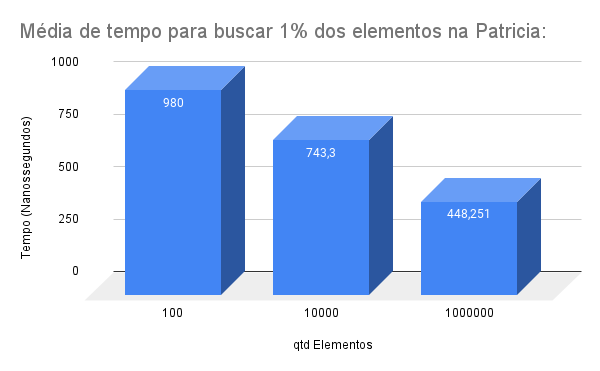
\includegraphics[scale=0.6]{Trabalho AED/fig/Média de tempo para buscar 1 dos elementos na Patricia_.png}
            \label{fig:Media de tempo Trie}
    \end{center}
    
\begin{center}
            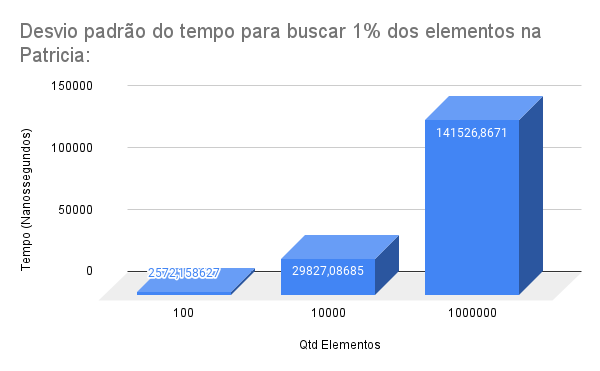
\includegraphics[scale=0.6]{Trabalho AED/fig/Desvio padrão do tempo para buscar 1 dos elementos na Patricia_.png}
            \label{fig:Media de tempo Trie}
    \end{center}